\textit{This chapter presents a method to create a repository to store the similarity between a large number of datasets involving the detection of duplicated datasets and dataset chunks. To this aim, we store those similarities, providing an index to store the relation among them. The similarities processing is based on thee properties and classes of each dataset. We give a similarity score to each dataset pair and also provide an search engine to find similar datasets, classes and properties for a given a given dataset, class or property.
We build the index over a total of 668,166 datasets from LOD Stats and LOD Laudromat as well as 559 active SPARQL endpoints. These data sources represent a total of 221.7 billion triples from more than 5 terabytes of information from datasets partially retrieved using the service ``Where is My URI'' (WIMU). Our evaluation on state-of-the-art real-data shows that more than 90\% of datasets from LODLaundromat datasets are not using owl:equivalentProperty and owl:equivalentClass or other way to relate the data, reinforcing the need for a index of relations among LOD datasets.}

\section{Introduction}
People will always describe the knowledge differently, due to the individuality of the being, different point of view, time and space, in which we assume as a natural phenomenon and standard. Aware of the state of the art from Ontology/Schema/Instance Matching from Linked Data from venues such as VLDB\footnote{\url{https://www.vldb.org/}}, OEAI\footnote{\url{http://oaei.ontologymatching.org/}}, ISWC\footnote{\url{https://iswc2019.semanticweb.org/}}, ESWC\footnote{\url{https://2019.eswc-conferences.org/}}, among others, we observe that the LOD datasets are following this standard.

We notice that there are several similar datasets. Still, there is no place that stores or provides such kind of information about how similar are the datasets or which attributes the datasets share. This work has the aim to build an index to store the relation among the datasets to have a place to see how similar are the datasets.
We provide a method to index the relation among LOD datasets\footnote{Datasets from LODStats, LODLaundromat, and endpoints} based on the properties and classes that they share.

We start giving two examples about how useful can be the index:

\textbf{Example 1}: Given the following SPARQL query, where the user wants to know if the dataset contains 3 properties, in which the user already know the query works well at the a SPARQL endpoing from CKAN\footnote{  CKAN SPARQL endpoint~\url{https://linked.opendata.cz/sparql}}:
\begin{verbatim}
Select * where { ?s ?p ?o.
Filter(?s=<http://purl.org/dc/terms/date> || 
?s=<http://crime.rkbexplorer.com/id/location> || 
?s=<http://purl.org/dc/terms/subject>
)}
\end{verbatim}
The following questions can be done:
\begin{itemize}
    \item How to know which datasets are able to execute the query?
    \item Which of the datasets contains the most valuable results?
    \item Can, the results from different datasets complement each other?
\end{itemize}

In this case an approach is needed to able the user to know more datasets to extract the required information. An index of dataset relations/similarities could be used to know that the query can be also be executed with results at \url{https://eu.dbpedia.org/sparql} but not at \url{http://dbpedia.org/sparql}, and we can execute at least in more 5 datasets also complementing the results.

\textbf{Example 2}: The user need information about cities from all datasets in your repository, more specifically datasets that are compatible with the class \url{http://dbpedia.org/ontology/City}.
We consider here that to execute such task manually on more than 600,000 datasets is not feasible. Thus, having an index of dataset relation will help in this case.

The contributions of this part of the thesis are:
\begin{itemize}
    \item A method to create an incremental index of similarity among LOD datasets. Thus, to the best of our knowledge, ReLOD is the first dataset relation index over a net total of 221.7 billion triples.
    \item A creation of a mechanism to search this index by Dataset URI, property, class or SPARQL query. For the first time, to the best of our knowledge, we make an relation index able to query by dataset URI, property, class or SPARQL query.
    \item An method to identify duplicated datesets and chunks.
\end{itemize}

The rest of this chapter is organized as follows:
\Cref{sec:approach} introduces our approach. \Cref{sec:eval} shows the evaluation results and discussion.

\section{The approach}
\label{sec:approach}
Our observations guide us to a method to create an index of LOD datasets, in which involves a compilation of many other works, starting collecting data from more than 650 thousand LOD datasets from LODStats and LODLaundromat and more than 500 endpoints. 

%Among the steps we should hightlight the creation of a \textbf{Dataset catolog}, section\ref{sec:lodCatalog}, providing an efficient way to obtain all properties and classes from each dataset and an \textbf{approach to identify the namespace} of each dataset, described at section\ref{sec:namespace}, avoiding the necessity to open each dataset in order to know what more the domain of the dataset.

\subsection{The index creation}
\label{sec:indexCreation}

Given a set of Datasets $\mathbf{D}\{d_1,...,d_n\}$, Assuming $d_n$ represents a RDF dataset\footnote{RDF datasets: \url{https://www.w3.org/TR/rdf11-datasets/}}, in which each $d$ contains a set of properties and classes represented by $\mathcal{P}$. The next step is done in a separated independent process, not interfering in the run-time of the index creation, in which consists in create a set $\mathbf{E}$ containing the identified duplicated datasets. Thus, we can exclude from $\mathbf{D}$ all datasets contained in $\mathbf{E}$.

The goal of algorithm \ref{alg:indexCreation}\footnote{Implementation in Java \url{https://tinyurl.com/y597qrah}} is to create an index to store the relations among datasets by comparing the occurrences of classes and properties of each dataset, by String similarity and Instance Matching. In this way, simplifying, the \textbf{Input} are a set of Datasets and the \textbf{Output} is the index of dataset relations.

The \cref{fig:create} show a workflow about how the index is created and the algorithm \ref{alg:indexCreation} describe with more details the process of creation of the  dataset relation index.

\begin{figure}[htb] 
	\centering
	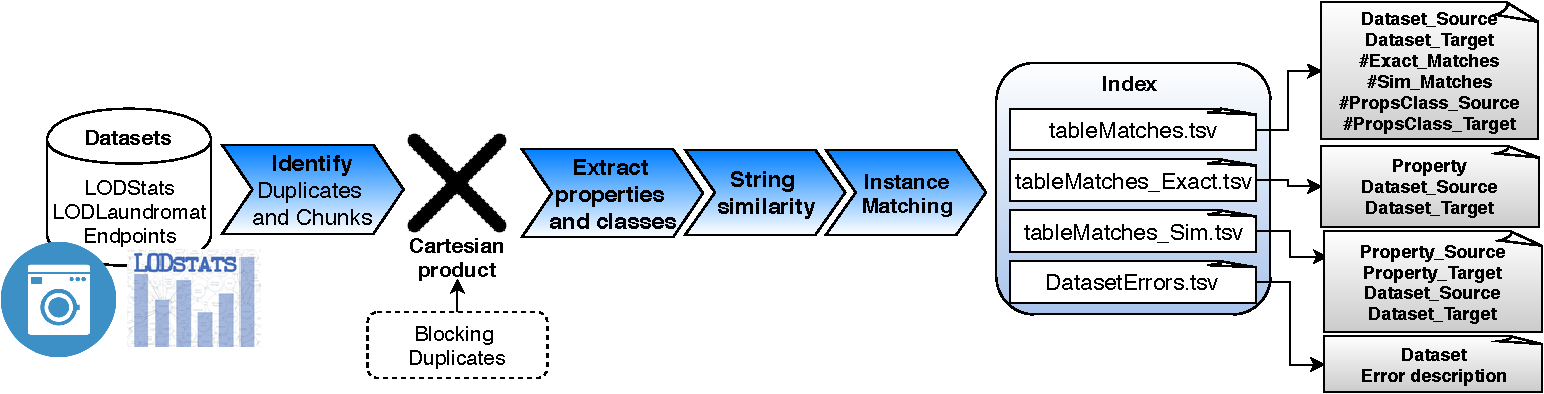
\includegraphics[width=\linewidth]{img/createIndex.pdf}
	\caption{Creating the index.}
	\label{fig:create}
\end{figure}

\begin{algorithm} [htb] 
	\caption{Creation of the LOD dataset relation index}
	\label{alg:indexCreation}
    %\begin{multicols}{2}
    	\textbf{Input}: $\mathbf{D}, \mathbf{E}$ \Comment{Datasets and datasets duplicated} \\
    	\textbf{Output}: $\mathbf{C}, \mathbf{X}, \mathbf{Y}, \mathbf{Z}$  \Comment{Four tsv files containing the matches(datasets, classes and properties).}
    	\begin{algorithmic}[1]
    	    \State{$\mathbf{M}_e \{\}$} \Comment{HashMap containing datasetTarget and another hash containing properties and classes exact matched}
    	    \State{$\mathbf{M}_s \{\}$} \Comment{HashMap containing datasetTarget and another hash containing properties and classes matched using String similarity}
    	    \State{$\mathbf{M}_a \{\}$} \Comment{HashMap containing datasets already compared}
    	    \State{$\mathbf{D}-\mathbf{E}$} \Comment{Remove duplicates contained in $\mathbf{E}$}
    	    \State{$\mathbf{T}=\mathbf{D}$}
    	    \ForAll{$\mathbf{d} \in \mathbf{D}$} \Comment{In parallel}
    	        \ForAll{$\mathbf{t} \in \mathbf{T}$}
        	        \If{($\mathbf{d}$ <> $\mathbf{t}$) $\land$ \textbf{alreadyCompared}($\mathbf{d},\mathbf{t}$)} 
        	            \State{continue} \Comment{Skip the current $\mathbf{d}$ and $\mathbf{t}$}
        	        \EndIf
        	        \State{$\mathbf{M}_e$.add(\textbf{getExactMatches}($\mathbf{d},\mathbf{t}$))} \Comment{Add a set containing the properties/classes that are exact the same in both datasets}
					\State{$\mathbf{M}_s$.add(\textbf{getSimMatches}($\mathbf{d},\mathbf{t}$, 0.8, $\mathbf{M}_e$))} \Comment{Add a set containing the properties that are similar in both datasets, excluding the matches from $\mathbf{M}_e$}
					\State{$\mathbf{M}_a$.add(d, t)} \Comment{Add the dataset pair already processed}
    	        \EndFor
    	    \EndFor
    	    \State{\textbf{printMaps}($\mathbf{M}_e, \mathbf{M}_s$)} \Comment{Print the content of $\mathbf{M}_e$ and $\mathbf{M}_s$ inside the files $\mathbf{C}, \mathbf{X}, \mathbf{Y}, \mathbf{Z}$}
    	\end{algorithmic}
    %\end{multicols}	
\end{algorithm}  

The function \textbf{getExactMatches}($\mathbf{d},\mathbf{t}$)) compares all properties and classes from each dataset $\mathbf{d}$ and $\mathbf{t}$ and return a set of properties and classes that are exact the same, keeping the provenance of the dataset.

The function \textbf{getSimMatches}($\mathbf{d},\mathbf{t}$, 0.8, $\mathbf{M}_e$) compares all properties and classes from each dataset $\mathbf{d}$ and $\mathbf{t}$ using Jaccard and MFKC\cite{valdestilhas2017high} String Similarity function with a threshold of 0.8, excluding the exact matches identified previously by the function \textbf{getExactMatches} returning the a set of properties and classes that has the similary greater than the threshold 0.8, keeping the provenance of the dataset, the \cref{fig:simMatch} shows our string similarity process.
\begin{figure}[htb] 
	\centering
	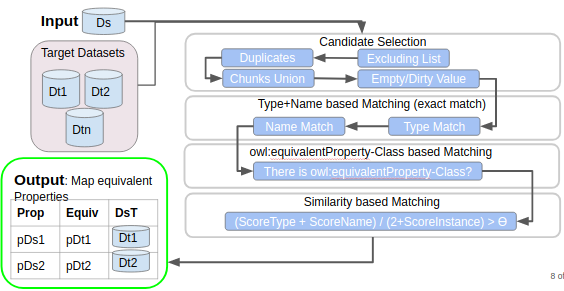
\includegraphics[width=\linewidth]{img/stringSim.png}
	\caption{String similarity process.}
	\label{fig:simMatch}
\end{figure}

The function \textbf{printMaps}($\mathbf{M}_e, \mathbf{M}_s$) print the content from the matching functions into the files according the structure described in section \ref{sec:FileStructure}.

\subsection{Identifying duplicated and chunk datasets}
\label{sec:duplicates}
With the current hardware available (HD 1Tb, Memory 16GB, processor intel core i7).
To compare all LOD datasets, in this case more than 600 thousand datasets, implies in more than 360 billion of comparisons($n*n$), assuming that each comparison takes in average 1 millisecond, the whole operation will take more than 10 years.

Thus, we need:
\begin{itemize}
    \item A blocking technique to avoid unnecessary comparisons. In this case we already have a way to detect duplicated and chunk-dump-files detection. A possible solution would be to create another index containing the elements to be blocked, such as datasets with less than 1 triple, duplicates, less than 5 properties, less than 5 classes.
    \item A better hardware.
\end{itemize}

The function \textbf{eliminateDuplicates()}, identify and eliminate duplicated HDT files by comparing the property occurrences of each dataset and the header metadata.

We formalize the problem of Clustering datasets identifying duplicates and chunks as follows:

We consider a set of $\mathbf{K}$ data sources $\mathbf{S_1}, . . . , \mathbf{S_k}$ containing property occurrences $\mathbf{O_1}, . . . , \mathbf{O_m}$. Each of property $\mathbf{P}$ is referenced by an \texttt{URI}, e.g., dbo:City\footnote{dbo:City states for the URI \url{http://dbpedia.org/ontology/City}}. Each $\mathbf{S}$ contains a header $\mathbf{H}$, with meta-data about the data in $\mathbf{S}$, such that $\mathbf{H} \subset \mathbf{S}$.

The goal is to create clusters of datasets $\mathbf{C}$ in two groups of elements from $\mathbf{K}$, in which are duplicates $\mathbf{D}$ and chunks $\mathbf{E}$, such that $\mathbf{D} \subset \mathbf{K} : \mathbf{E} \subset \mathbf{K} : \mathbf{K} \subset \mathbf{C}$.

We assume that all datasets are not empty and are RDF compatible with the HDT format.

Firstly we create a dense matrix of property occurrence and dataset. Then it was observed a standard in the dense matrix, that for some datasets the occurrence of the properties was exactly the same. Then, we identify that we can put together those datasets to observe more characteristics.
In this second phase, we have a sub-collection of our initial collection of datasets and looking into the header metadata of those files we observe that for some files the meta-data is different. Then we have another sub-collection of files with different headers, and manually reading file by file we realize that they are chunks, in other words, part of a bigger dataset. 

Thus we can have two phases for clustering dataset (1) Put together datasets that present the same occurrence of properties. (2) Read the header metadata and separate files with a different header. The files with different header are chunks and the rest are duplicates\footnote{More details, please see the implementation and the documentation on \url{https://github.com/firmao/wimuT} and the specific implementation java class for this task: \url{https://github.com/firmao/wimuT/blob/master/src/org/wimu/datasetselection/parallelv1/ClusterKmeans.java}}.

% \begin{figure}[htb] 
% 	\centering
% 	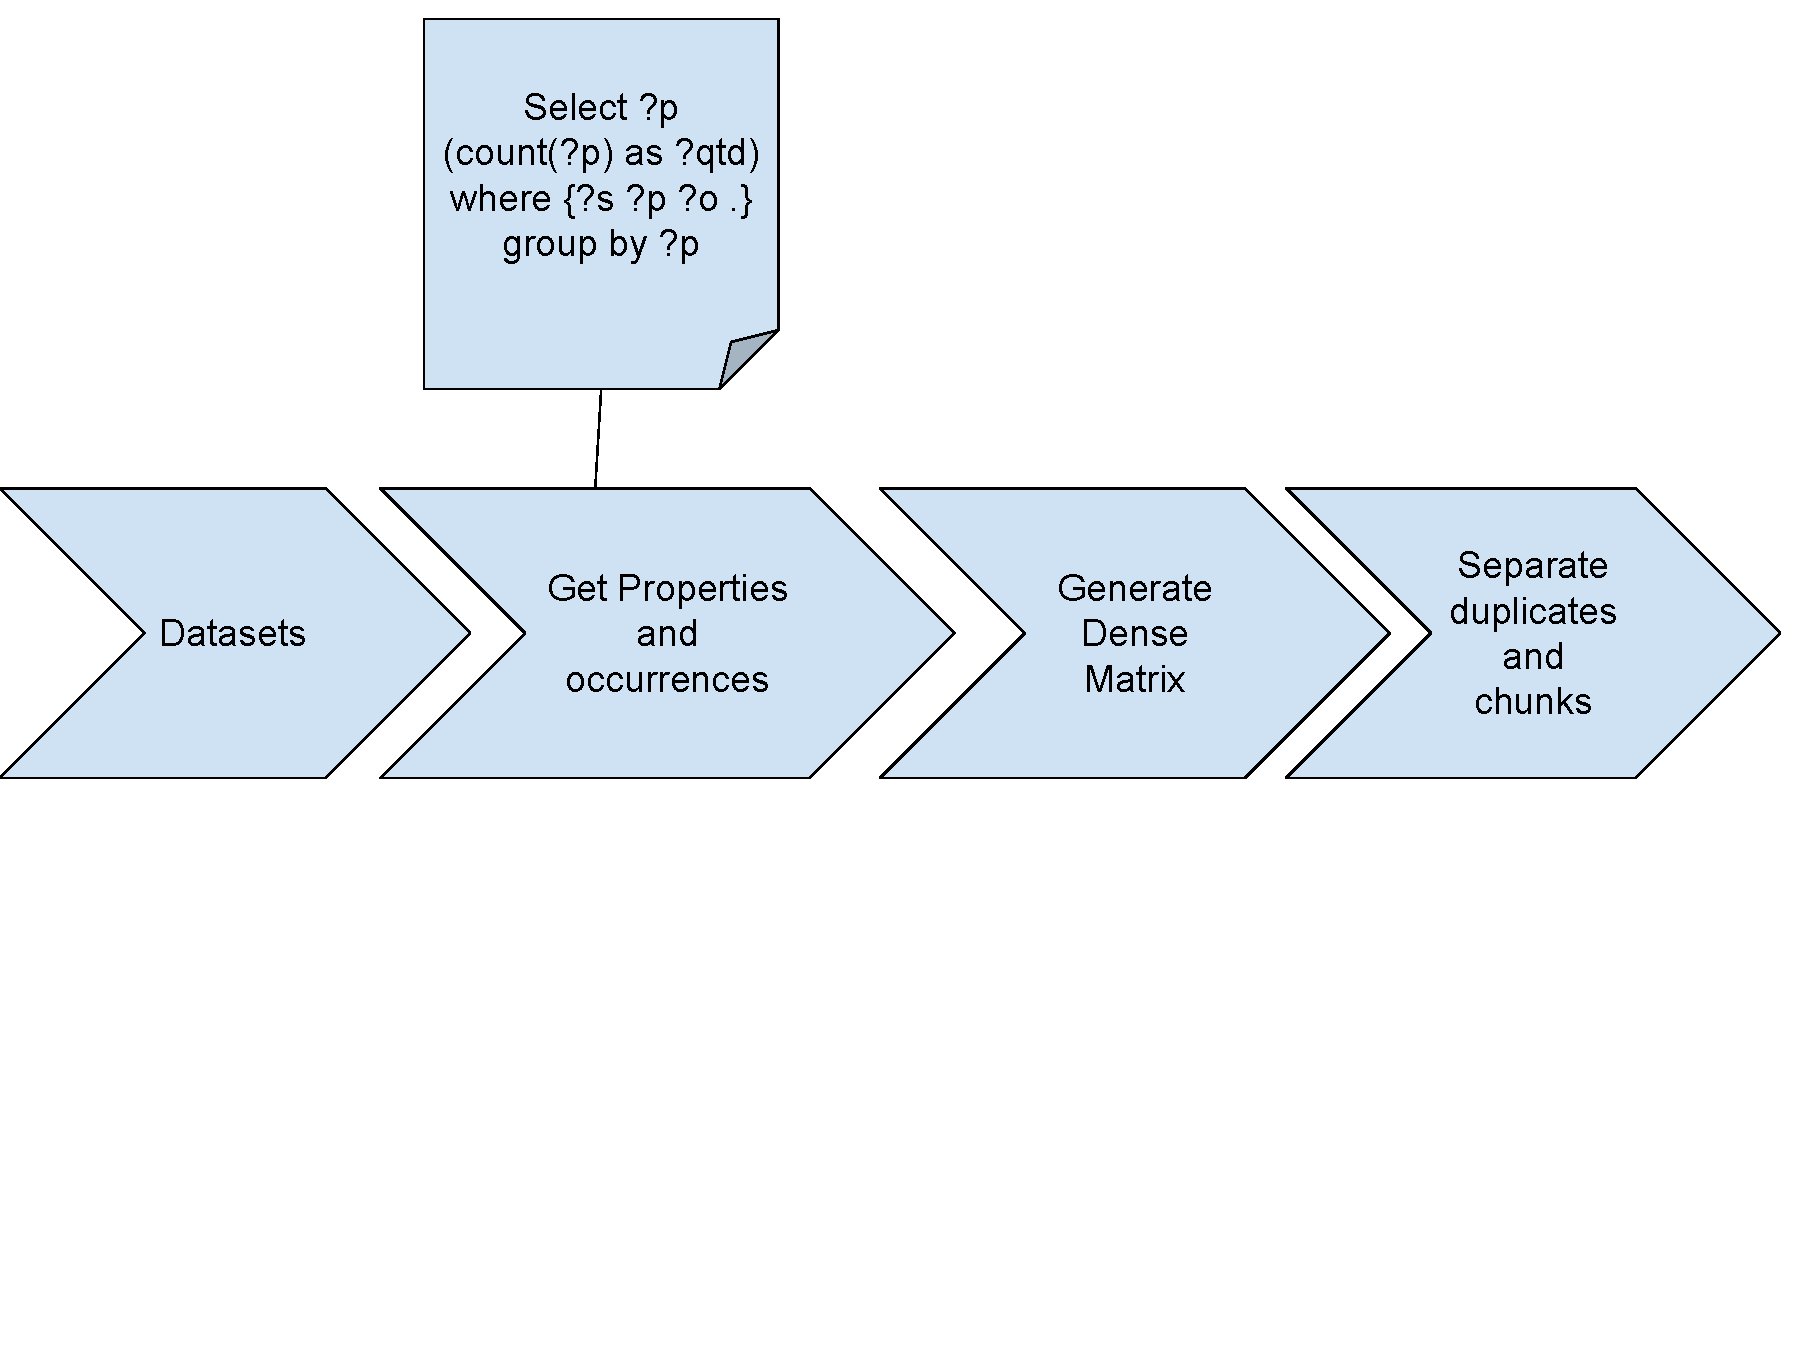
\includegraphics[width=\linewidth]{img/duplicates.pdf}
% 	\caption{Identifying duplicates and chunks.}
% 	\label{fig:duplicates}
% \end{figure}

\begin{algorithm} [htb] 
	\caption{Identifying duplicates and chunk}
	\label{alg:iss1}
    %\begin{multicols}{2}
    	\textbf{Input}: $\mathbf{D}$ \Comment{Datasets} \\
    	\textbf{Output}: $\mathbf{C}, \mathbf{X}$  \Comment{two files chunks.txt and duplicates.txt.}
    	\begin{algorithmic}[1]
    	    \State{sep = $\mathbf{t}$} \Comment{Separator for the file, in this case, a tab, but could be another such as “,”, etc..}
    	    \State{setHeader = $\{\}$}
    	    \State{cSparql = “Select ?p (count(?p) as ?qtd) where {?s ?p ?o .} group by ?p”}
    	    \ForAll{$\mathbf{d} \in \mathbf{D}$}
    	        \State{H = getPropertyOccurrence(ds)}
    	        \ForAll{$\mathbf{key,value} \in \mathbf{H}$} \Comment{\textbf{key} represent the property and \textbf{value} represents the number of occurrences.}
    	            \State{setHeader.add(key)}
    	            \State{line = line + sep + value}
    	        \EndFor
    	        \State{printLineDenseMatrix(d + line)}
    	        \If{setLines.contains(line)} \Comment{Here we identify and put chunks and duplicates together}
    	            \State{$\mathbf{D’}$.add(d)}
    	        \Else
    	            \State{setLines.add(line)}
    	        \EndIf
    	    \EndFor
    	    \State{printHeaderDenseMatrix(setHeader)}
    	    \State{$\mathbf{C}$.add(diff($\mathbf{D’}$))} \Comment{Here we separate chunks and duplicates}
    	    \State{$\mathbf{X}$.add(diffD($\mathbf{D’}$))}
     		\State{return $\mathbf{C}, \mathbf{X}$} \Comment{two files chunks.txt and duplicates.txt.}
    	\end{algorithmic}
	%\end{multicols}
\end{algorithm}    	

The function \textbf{getPropertyOccurrence}(ds) returns a hash map containing the property and the number of occurrences of each property from a given dataset with the following SPARQL query \textit{“Select ?p (count(?p) as ?qtd) where {?s ?p ?o .} group by ?p”}.
The function \textbf{printLineDenseMatrix}(line) print a line in a file and the function \textbf{printHeaderDenseMatrix}(setHeader) print the first line of the dense matrix file containing the header of the matrix, in which refers to the identification of the properties.
The function \textbf{diff}($\mathbf{D’}$ ) separates the chunks from duplicates, for this task we look into the header of the files, in this case, only HDT files, where duplicates present exactly the same header metadata information and chunks are different respect to the header.

\textbf{Theorem 1}: Let $\mathbf{P}$ be a collection of property occurrences of datasets $\mathbf{D}$, such that each $\mathbf{D}$ has one $\mathbf{P}$, in which $\mathbf{D’}$ represents the cluster candidates, in which are the datasets identified as chunks and duplicates together, and the function \textbf{diff()} return the dump-files that are not duplicated. Thus, the output of Algorithm 1 when applied to $\mathbf{D}$, the following hold:

$|\textbf{diff}(\mathbf{D’})| = 0$

All elements from D’ are duplicated datasets.


To identify the chunks:

$|\textbf{diff}(\mathbf{D’})| > 0$


The result from $\textbf{diff}(\mathbf{D’})$ are the dump-files identified as chunks.

% \subsection{The LOD catalog - Class property index}
% \label{sec:lodCatalog}
% \todo[inline]{Claus, when you are ready let's put your work here and some experiments/evaluation later. I also need to adapt my code to yours.}

% \subsection{Relating the name spaces with dataset names}
% \label{sec:namespace}
% The datasets from LODLaundromat\cite{} are identified with a MD5 code\footnote{ref MD5}, e.g \texttt{009e80050fa7f4279596956477157ec2.hdt}\footnote{\url{http://139.18.13.76:8082/dirHDTLaundromat/decompressed/00/009e80050fa7f4279596956477157ec2/009e80050fa7f4279596956477157ec2.hdt}} represent a dataset from the domain \texttt{knoesis.wright.edu} in which is a dataset about \textit{The Ohio Center of Excellence in Knowledge-enabled Computing (Kno.e.sis)}.

% We developed a method to convert the MD5 code from the HDT to URLs with more informative name spaces, instead of the MDA code we have the name space of the dataset giving us more information about the dataset avoiding the need to open the HDT file to obtain this information.

% The Algorithm \cref{alg:Edgard} describes how we create this complementary index.

% \todo[inline]{Edgard, please describe the algorithm when is better for you. And some evaluation.}

% \begin{table}[]
% \begin{tabular}{@{}lcccc@{}}
% \toprule
% \textbf{Process}           & \multicolumn{1}{l}{\textbf{Runtime}} \\ \midrule
%  Complete Namespace extraction & ?             \\              
%  Dominant Namespace extraction & ?             \\              Index creation    & ?               \\
%  \bottomrule
% \end{tabular}
% \end{table}

\subsection{The file structure}
\label{sec:FileStructure}

The file structure of the index is only 3 TSV files.
\begin{itemize}
    \item $\textbf{tableMatches\_Exact.tsv}$: Contains the exact match of the properties, with the following fields: 
    \begin{itemize}
        \item \textbf{Property}: containing the property URI itself.
        \item \textbf{Source}: Contains the dataset source where the property was found.
        \item \textbf{Target}: Contains de dataset matched containing the property.
    \end{itemize}
    \item $\textbf{tableMatches\_Sim.tsv}$: Represents the similarity of properties from datasets Source and Target, with the following fields:
    \begin{itemize}
        \item \textbf{PropertyS}: The property from the dataset Source.
        \item \textbf{PropertyT}: The property from the dataset Target.
        \item \textbf{Source}: The dataset Source.
        \item \textbf{Target}: The dataset Target.
    \end{itemize}
    \item \textbf{tableMatches.tsv}: Represents the datasets Matched and his respectives number of properties exact matched and number of properties matched with String similarity, with the following fields:
    \begin{itemize}
        \item \textbf{Source}: The dataset source.
        \item \textbf{Target}: The dataset Target.
        \item $\textbf{\#ExactMatch}$: Number of properties with exact match.
        \item $\textbf{\#sim>0.9}$: Number of properties with similarity threshold greater than 0.9.
    \end{itemize}
\end{itemize}

\subsection{Querying the index}
%\todo[inline]{Describe how to query the index, how the web prototype do the task: \url{https://github.com/firmao/LODDatasetRelationsWeb}} 

The index provides the following information based on three types of input:
\begin{description}
    \item \textbf{Dataset}: The index will provide a list of datasets, number of exact matched\footnote{Exact Match where the URI is exact the same following the principle of uniqueness of the URI} properties and number of similar\footnote{Similarity match occurs when the similarity of the URI is greater than 0.9 if less we perform Instance matching.} properties.
    \item \textbf{Set of properties (URIs) separeted by comma}: 
    \begin{itemize}
        \item Json file containing the property and the list of datasets where this property were found by exact match.
        \item A table containing the matches by similarity with the following fields:
        \begin{description}
            \item \textbf{Property Source}: Representing the property found on the dataset source.
            \item \textbf{Property Target}: Representing the property found on the dataset target.
            \item \textbf{Dataset Source}: The name of the dataset source.
            \item \textbf{Dataset Target}: The name of the dataset target.
        \end{description}
    \end{itemize}
    \item \textbf{SPARQL query}: This type of input extracts the set of properties from the SPARQL query and performs the same operation as \textbf{Set of properties (URIs) separeted by comma}.
\end{description}

\begin{figure}[htb] 
	\centering
	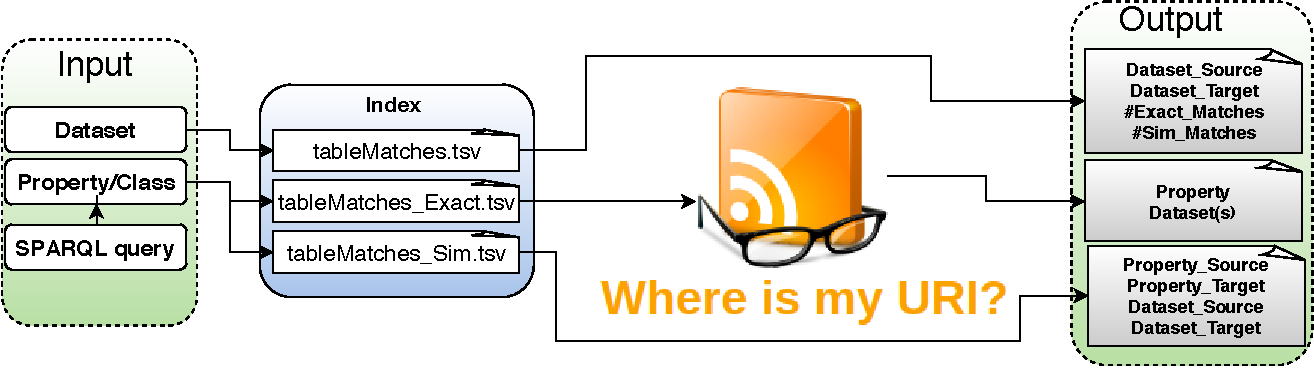
\includegraphics[width=\linewidth]{img/queryIndex.pdf}
	\caption{Querying the index.}
	\label{fig:queryIndex}
\end{figure}

The index is incremental, allowing to add more datasets to be processed once a month\footnote{Once a month due to the the time to generate that with our hardware takes at least 88 hours}.
The prototype is available online for proof of concept online\footnote{\url{http://w3id.org/relod/}} and the \cref{fig:queryIndex} shows a workflow about how the index is used.

% \todo[inline]{try with elasticsearch and see if is better or not.}
% \begin{verbatim}
% elasticsearch_loader <options> csv --delimiter '\t' filename.tsv

% https://www.reddit.com/r/elasticsearch/comments/at7huu/how_can_i_import_tsv_to_elasticsearch/
% \end{verbatim}

%The \cref{fig:datasetMatch},\cref{fig:exactMatch}, \cref{fig:similarMatch} show 3 examples of 3 different types of results to 3 different queries to the index.

% \begin{figure}[htb] 
% 	\centering
% 	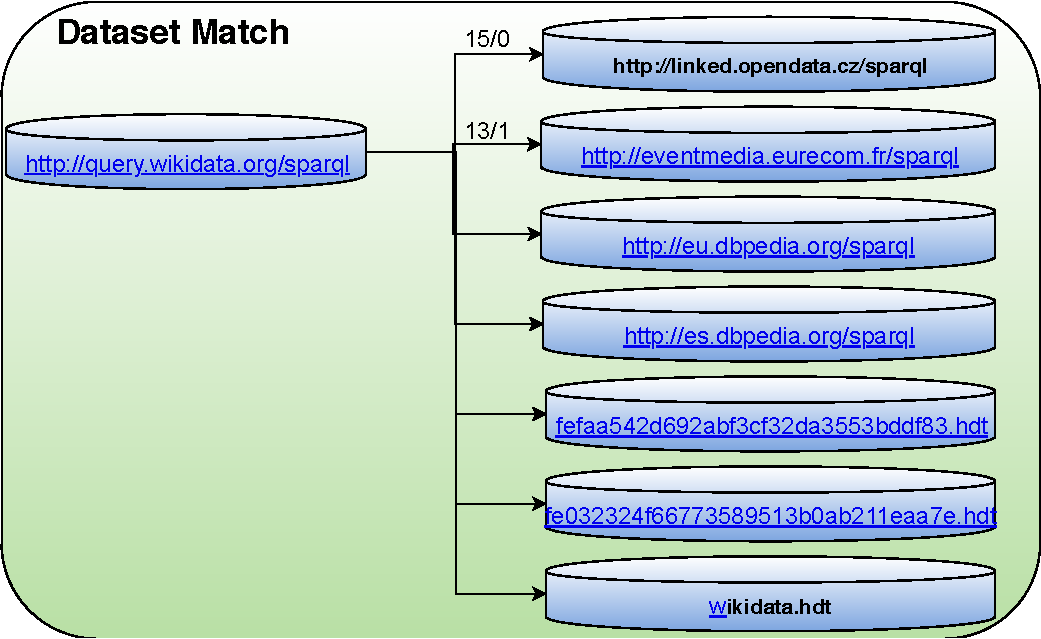
\includegraphics[width=\linewidth]{llncs/img/datasetMatch.pdf}
% 	\caption{Example of dataset match.}
% 	\label{fig:datasetMatch}
% \end{figure}

% \begin{figure}[htb] 
% 	\centering
% 	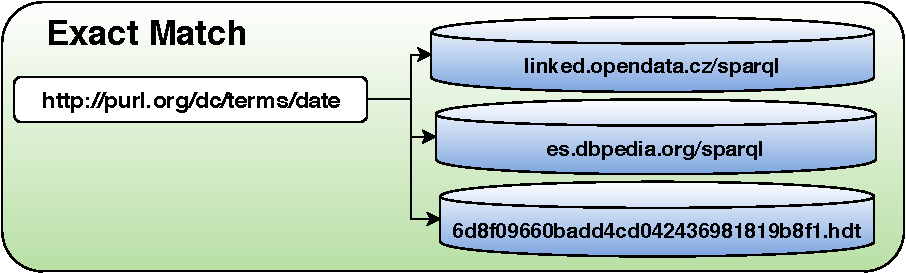
\includegraphics[width=\linewidth]{llncs/img/exactMatch.pdf}
% 	\caption{Example of exact match.}
% 	\label{fig:exactMatch}
% \end{figure}

% \begin{figure}[htb] 
% 	\centering
% 	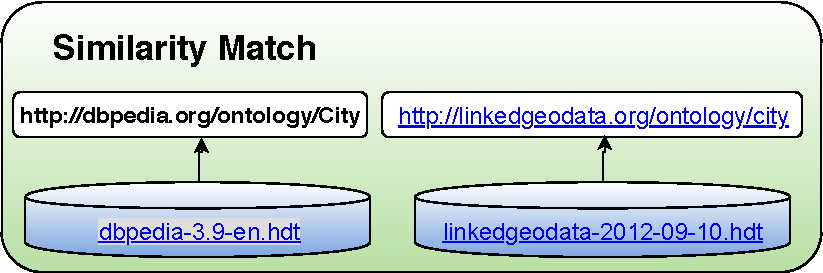
\includegraphics[width=\linewidth]{llncs/img/similarMatch.pdf}
% 	\caption{Example of similar match.}
% 	\label{fig:similarMatch}
% \end{figure}

\section{Evaluation}
\label{sec:eval}
% The evaluation aims to answer the following questions: (1) How to identify and quantify similar datasets for a given Dataset?\footnote{To know how many datasets are similar to each other.} (2) How many datasets are most likely to execute a given SPARQL query? (3) How many datasets you should read the content to know the domain and namespace? (4) How the detection of duplicated and chunk datasets can help in the process of matching a large amount of datasets?
The evaluation aims to answer the following questions: (1) How to identify and quantify similar datasets for a given Dataset?\footnote{To know how many datasets are similar to each other.} (2) How many datasets are most likely to execute a given SPARQL query? (3) How the detection of duplicated and chunk datasets can help in the process of matching a large amount of datasets?

To answer the question (1) we give to our approach as input a version of the dataset DBpedia\footnote{\url{http://gaia.infor.uva.es/hdt/DBPedia-3.9-en.hdt.gz}}, that contains 2339 properties and classes, and as output we can obtain the most similar datasets\footnote{We compare with the datasets from \url{http://www.rdfhdt.org/datasets/}}. Thus we sorted those datasets in a way of Top 10 datasets more similar to DBpedia, according to the properties and classes they share. On the \cref{tab:top10} we show the number of properties that they share that contains the exact same URI and cases where they share not the exact URI but very similar\footnote{With similarity level greater than 0.8 according our similarity algorithm.}. Thus, an example of application could with a case when the user wants to identify information from other datasets to complement or enrich information for a given dataset, i.e. facilitating federated queries. The \cref{tab:match} shows a evaluation with 600 randonly chosen datasets\footnote{European statistics: HDT files from LOD Laundromat: Economic accounts for agriculture (aact) - \url{http://ec.europa.eu/eurostat/cache/metadata/en/aact_esms.htm}} including 3 synthetic manually made datasets.

\begin{table}[htb]
\begin{tabular}{lcccccccccccc} \hline
\textbf{Dataset} & \textbf{\#ExactMatch} & \textbf{\#sim > 0.8} & \textbf{\#PropClas}s \\  \hline
swdf-2012-11-28.hdt & 22 & 64 & 288 \\
yago2s-2013-05-08.hdt & 6 & 65 & 373546 \\
dblp-20170124.hdt & 6 & 9 & 41 \\
linkedgeodata-2012-09-10.hdt & 5 & 617 & 11799 \\
wiktionary_en_2012-07-21.hdt & 4 & 6 & 31 \\
geonames-11-11-2012.hdt & 4 & 12 & 27 \\
wordnet31.hdt & 3 & 26 & 69 \\
wikidata-20170313-all-BETA.hdt & 0 & 5 & 427 \\
freebase-rdf-2013-12-01-00-00.hdt & 0 & 55 & 17587 \\ \hline
\end{tabular}
\caption{Top 10 datasets containing exact the same URI and containing the most similar URIs according to our similarity approach, in which \#PropClass represents the total number of properties and classes from the dataset. }
\label{tab:top10}
\end{table}

\begin{table}[htb]
    \centering
    \begin{tabular}{ccccc}
    \textbf{\#Datasets} & \textbf{\#DatasetsPropMatch} & \textbf{time (seconds)} & \textbf{\#triples} & \textbf{Synthetic} \\
    3 & 2 & 1 & 11 & Yes \\
    10 & 7 & 2 & 1198508 & no \\
    100 & 39 & 12 & 7996408 & no \\
    200 & 92 & 40 & 22982984 & no \\
    300 & 135 & 57 & 34792121 & no \\
    400 & 186 & 73 & 43864522 & no \\
    500 & 229 & 87 & 54227780 & no \\
    600 & 291 & 425 & 85041239 & no \\
    \end{tabular}
    \caption{Evaluation on the Match algorithm, where \textbf{DatasetsPropMatch} refers to the number of properties/classes the datasets share among each other.}
    \label{tab:match}
\end{table}

Observing the \cref{fig:match600Laundromat} we could estimate that around 50\% of the properties and classes has a match in another dataset, showing the high possibility to one dataset could enrich each other. 

\begin{figure}[htb] 
	\centering
	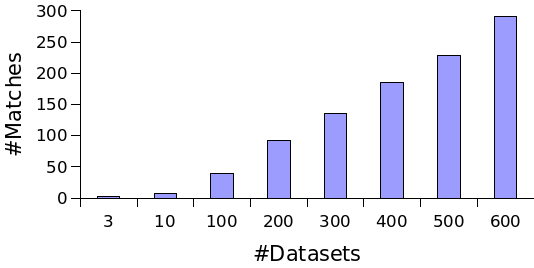
\includegraphics[width=\linewidth]{img/LaundromatDsMatch.png}
	\caption{Dataset Matching (600 datasets LODLaundromat).}
	\label{fig:match600Laundromat}
\end{figure}

\begin{figure}[htb] 
	\centering
	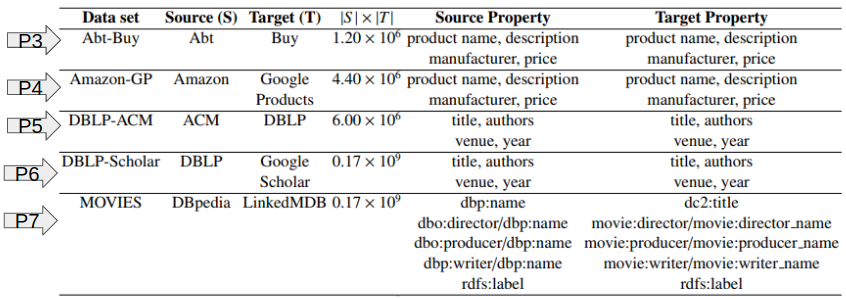
\includegraphics[width=\linewidth]{img/goldESWCKleanthi.png}
	\caption{Sample datasets from \cite{georgala2018dynamic} to evaluate our string similarity approach.}
	\label{fig:TableFmeasure}
\end{figure}

The time consumed can be observed on \cref{fig:time600Laundromat}, which shows that 100 million triples were processed in less than 8 minutes, in which is a acceptable time, in which the starts to be time-consuming only after 1 million triples.

\begin{figure}[htb] 
	\centering
	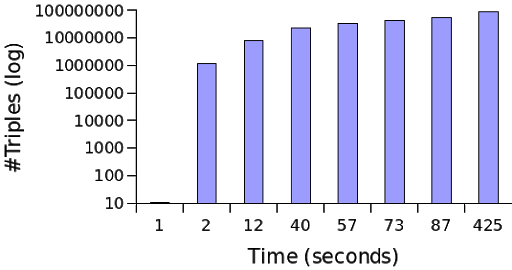
\includegraphics[width=\linewidth]{img/time.png}
	\caption{Time Dataset Matching (600 datasets LODLaundromat).}
	\label{fig:time600Laundromat}
\end{figure}

As we are using WimuQ\cite{valdestilhas2019more} to identify datasets for a given SPARQL query together with our matching algorithm, we can answer the question (2) based on famous Sparql queries from two real-data federated SPARQL querying benchmarks \emph{LargeRDFBench} \cite{largerdfbench2017},\emph{FedBench} \cite{fedbench2011} and one non-federated real data SPARQL benchmark selected from \emph{FEASIBLE} \cite{feasible2015} benchmarks generation framework is given in Figure \ref{fig:numberDatasets1}. Thus, from the selected datasets we use our approach to select the datasets according to the properties and classes they share among them\footnote{In this case, all datasets identified by wimuQ are sharing properties and classes, that is why we are using the graph from \cite{valdestilhas2019more}.}.
\begin{figure}[htb]
\centering
    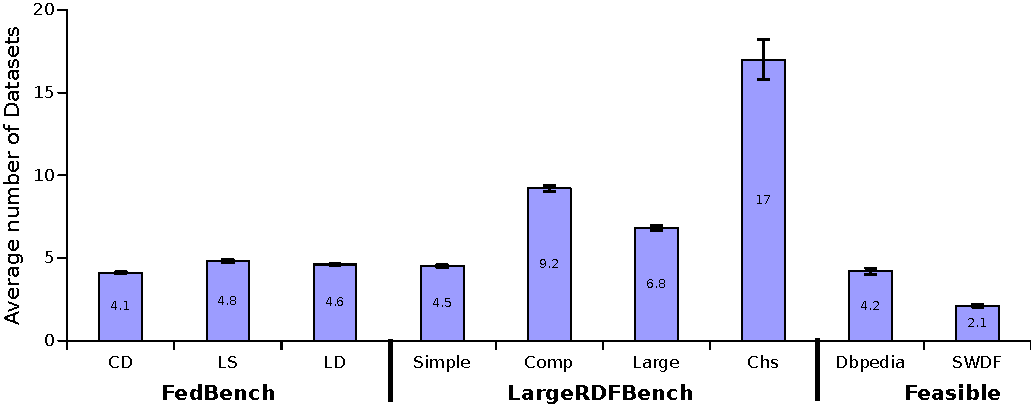
\includegraphics[width=\linewidth]{img/numberDatasets1.pdf}
	\caption{Average number of datasets discovered and queried by WimuQ\cite{valdestilhas2019more} across different queries categories of the selected benchmarks.}
	\label{fig:numberDatasets1}
\end{figure}

% To answer the question (3) we have the \cref{fig:md5Namespace} in which we can observe that all datasets from LODLaundromat are named with a MD5 code in which thanks to our approach you can know the domain and namespace information. There are \textbf{X} datasets from LODStats and \textbf{Y} SPARQL endpoints. \todo[inline]{Edgard, please verify and if not created yet, please create a graph/plot/chart fig:md5Namespace containing the info.}

To answer the question (3) we evaluate the dataset duplicated detection algorithm and the detection of dataset chunks.
From a 5446 datasets\footnote{A subset from those 600 datasets chosen previously} our algorithm detected 2272 duplicates and 1470 chunks in 3 hours.

The \cref{fig:identDuplicates} shows a case with 900 datasets chosen randomly, where we identified in 10 cases in which we can see the difference 

The \cref{fig:identChunks} show how many chunks we were able to identify among our sample data, in which lead us to know how segregated is data analysed, giving also the chance to know the complete dataset after the union of all chunks.

\begin{figure}[htb] 
	\centering
	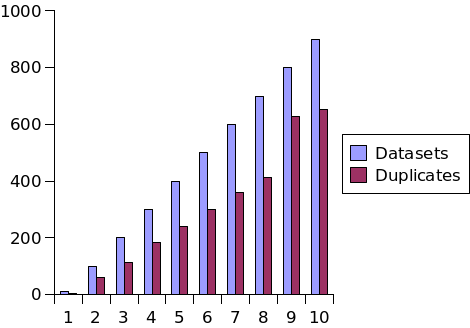
\includegraphics[width=\linewidth]{img/DsDuplicate.png}
	\caption{Duplicates identified in 900 datasets. Y axis represents the number of datasets.}
	\label{fig:identDuplicates}
\end{figure}

\begin{figure}[htb] 
	\centering
	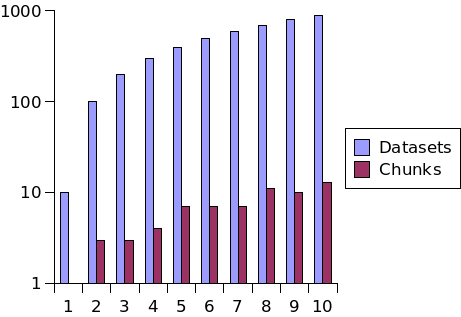
\includegraphics[width=\linewidth]{img/DsChunks.png}
	\caption{Chunks identified in 900 datasets. Y axis represents the number of datasets.}
	\label{fig:identChunks}
\end{figure}

The current version of the index prototype has information about 539 SPARQL endpoints from LOD cloud\footnote{The list of is available here: \url{https://github.com/firmao/wimuT/blob/master/Endpoints_numtriples_lodcloud.csv}} and 915 HDT files from LOD Laundromat\footnote{fdsa}. We perform more than 1,800,000 comparisons in 88 hours.

Where \textbf{DatasetsPropMatch} on the \cref{tab:match} refers to the number of properties/classes the datasets share among each other.

We can observe the quantity of properties/classes that the datasets share related to the number of triples analysed. For instance, from 600 datasets, 291 matches where found, in which the number of triples was almost the double size of the previous case. Thus, the number of matches in this case cannot be directly related to the number of triples. Due to this fact, the quality of the datasets should be considerate a important phase.

We evaluate the accuracy of our matching algorithm with a small sample, where we can see at \cref{fig:fmeasure}, \cref{fig:TableFmeasure} and \cref{runtimeSimilarMatch} the F-Measure and run-time on six famous pairs of datasets from\cite{georgala2018dynamic}, with those datasets we create a gold standard to compare, in which $P_1...P_n$ represents the pair of datasets and P1, P2 are datasets synthetically generated by the author, i.e. P3 represents the comparison between the datasets Abt and Buy.

\begin{figure}[htb] 
	\centering
	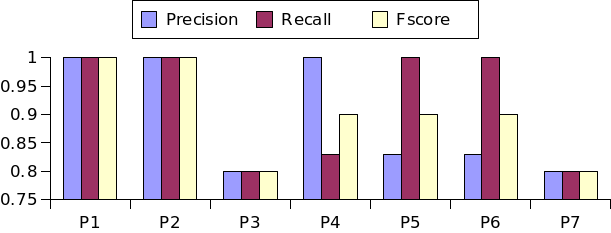
\includegraphics[width=\linewidth]{img/fmeasure.png}
	\caption{F-measure our string similarity.}
	\label{fig:fmeasure}
\end{figure}

\begin{figure}[htb] 
	\centering
	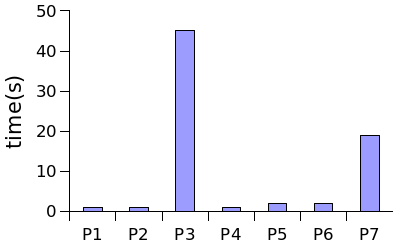
\includegraphics[width=\linewidth]{img/runtime.png}
	\caption{Runtime of our string similarity.}
	\label{fig:runtimeSimilarMatch}
\end{figure}

The \cref{fig:dumps} shows that the majority of files from LODStats are in RDF/XML format.
Moreover, the endpoints are represented in greater numbers (78.6\%), the dominant file format is RDF with 84.1\% of the cases, and 56.2\% of errors occurred because Apache Jena was not able to perform SPARQL queries.
Among the HDT files from LOD Laundromat, 2.3\% of them could not be processed due to parsing errors.
Another relevant point is that 99.2\% of the URIs indexed with WIMU come from LOD Laundromat, due to 69.8\% of datasets from LODstats contain parser errors in which WIMU was not able to process the data.
%https://docs.google.com/spreadsheets/d/15kh8E4WllXG5Xdp1aL-JiHvnXAiVC6a8XqVUJ1gtMZ8/edit?usp=sharing

\begin{figure}[htb] 
	\centering
	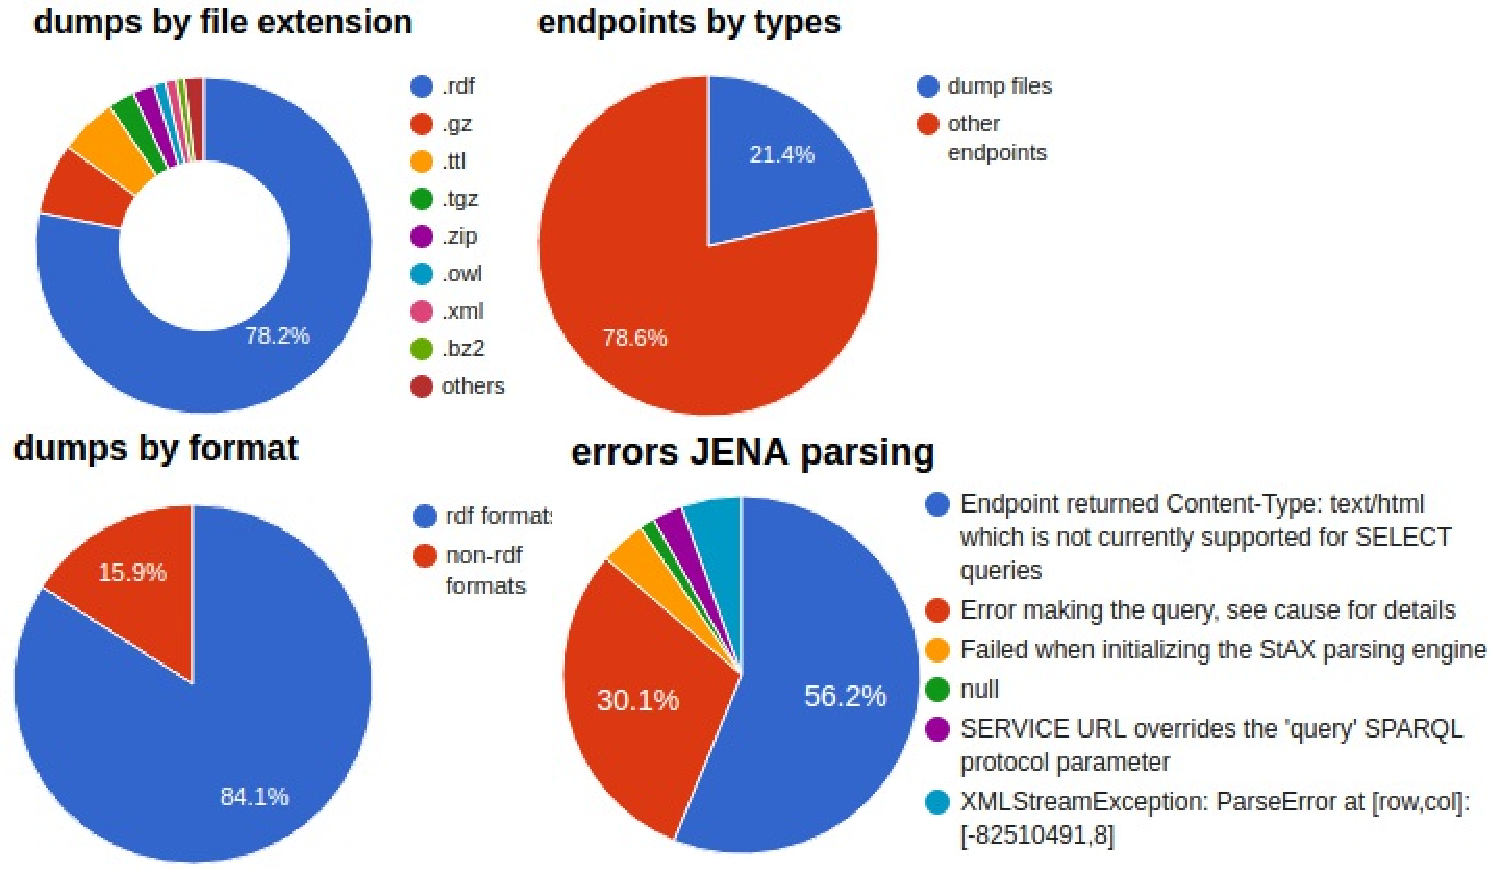
\includegraphics[width=1.0\linewidth]{img/dumps3.pdf}
	\caption{Dump files and Apache Jena parsing error.}
	\label{fig:dumps}
\end{figure}